\chapter{Реализация}
\label{chap:impl}

\section{Языковой сервер \Rzk{} и расширение для VS Code}

Описываем реализацию языкового сервера и расширения для \Rzk{} в среде VS Code.
Языковой сервер имеет прямой доступ к внутренностям доказательного ассистента,
включая алгоритм проверки типов и внутреннее абстрактное синтаксическое представление,
и предоставляет интерфейс, соответствующий протоколу языкового сервера.
Расширение для VS Code действует как посредник между редактором и языковым сервером,
предоставляя интерактивные возможности пользователю.

\subsection{Особенности}

Мы рассматриваем поддержку языкового сервера следующих особенностей.

\subsubsection{Интуитивный интерфейс и подсветка синтаксиса}

Расширение для VS Code предлагает интуитивно понятный интерфейс,
соответствующий ожиданиям математиков и компьютерных учёных.
Пользователи получают ясную и доступную навигацию,
позволяющую эффективно исследовать структуры, основанные на HoTT.
Кроме того, расширение обеспечивает подсветку синтаксиса и семантики,
улучшая читаемость кода и облегчая обнаружение ошибок.

\begin{figure}[ht]
  \centering
  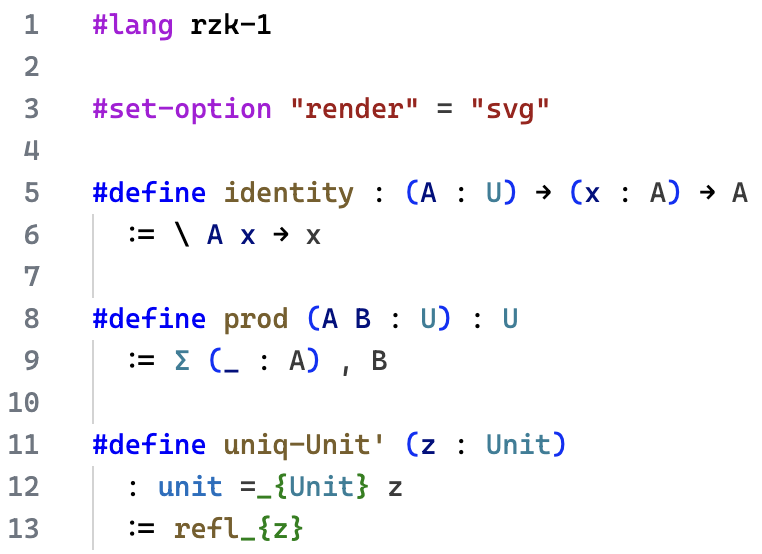
\includegraphics[width=0.7\textwidth]{figs/syntax-highlighting.png}
  \caption{Подсветка синтаксиса/семантики в VS Code.}
  \label{figure:syntax-highlighting}
\end{figure}

\subsubsection{Автодополнение кода и предложения}

Расширение для VS Code \Rzk{} использует LSP для предложения интеллектуального
автодополнения кода и предложений, основанных на контексте. В процессе работы
с \Rzk{} расширение помогает писать код более эффективно, предоставляя
соответствующие предложения, снижая вероятность синтаксических ошибок и
ускоряя процесс разработки.

\subsection{Расширение для VS Code}

Для предоставления пользователю указанных функций необходимо использовать тонкий обёртку вокруг языкового сервера в виде расширения для VS Code. Дополнительно расширение управляет установкой самого языкового сервера на всех основных операционных системах (Windows, macOS и Ubuntu) с использованием предварительно собранных бинарных файлов, прикреплённых к релизам на GitHub, а также обеспечивает сборку языкового сервера из исходного кода на платформах, для которых предварительно собранные бинарные файлы недоступны. Исходный код расширения доступен в репозитории GitHub\footnote{\url{https://github.com/rzk-lang/vscode-rzk}}, а само расширение доступно на платформе Visual Studio Marketplace\footnote{\url{https://marketplace.visualstudio.com/items?itemName=NikolaiKudasovfizruk.rzk-1-experimental-highlighting}} и на реестре Open VSX\footnote{\url{https://open-vsx.org/extension/NikolaiKudasovfizruk/rzk-1-experimental-highlighting}}, а также предварительно собранный бинарный файл на странице релизов GitHub\footnote{\url{https://github.com/rzk-lang/vscode-rzk/releases}}.

\subsubsection{Установка и активация}

После активации расширение проверяет доступность исполняемого файла \Rzk{} в переменной среды \texttt{PATH} системы. Если файл недоступен, расширение проверяет наличие загруженного ранее бинарного файла в локальном хранилище расширения. Если ни то, ни другое не найдены, пользователю предлагается скачать последнюю совместимую версию бинарного файла с страницы релизов GitHub и сохранить его в локальном хранилище. Пользователь может изменить это поведение, указав пользовательский путь к бинарному файлу языкового сервера.

Для загрузки предварительно собранного бинарного файла \Rzk{} расширение запрашивает доступные релизы на GitHub и находит последний релиз, совместимый с установленной версией расширения. Совместимость определяется с помощью диапазона версий в семантическом формате\cite{Preston2013semantic}, заданном в исходном коде расширения, и используется для фильтрации релизов и поиска последнего, удовлетворяющего заданному диапазону.

Затем расширение загружает бинарный файл с помощью SDK Octokit и извлекает tar-архив в локальное хранилище. После этого расширение просто запускает языковой сервер в отдельном процессе и устанавливает соединение с ним, остальное обрабатываются VS Code и языковой сервером.

\subsubsection{Настройка}

Расширение предоставляет пользователю опции конфигурации для настройки поведения расширения. Пользователь может указать путь к исполняемому файлу \Rzk{}, что полезно для пользователей, у которых исполняемый файл установлен в нестандартном местоположении, а также для тестирования. Пользователь также может включить или отключить функцию форматирования и выбрать, получать ли предварительные версии \Rzk{}.

Это достигается с помощью поля конфигурации\footnote{\url{https://code.visualstudio.com/api/references/contribution-points\#contributes.configuration}} в файле \texttt{package.json} расширения.

\subsection{Языковой сервер \Rzk{}}

В центре инструментального комплекса \Rzk{} находится языковой сервер, который обеспечивает все функции редактора, сделав разработку доказательств в \Rzk{} приятной. В настоящее время он поддерживает семантическую подсветку, диагностические сообщения и автодополнение текста. Также в разработке находится функция отчётности о ходе длительных процессов (например, проверка типов для больших проектов).

Первоначально языковой сервер поставляется вместе с доказательным ассистентом \Rzk{} как отдельная подкоманда, но планируется разделение этих компонентов и зависимость языкового сервера от основной библиотеки. Они реализованы на языке программирования Haskell с использованием пакета \texttt{lsp}\footnote{\url{https://hackage.haskell.org/package/lsp}}.

Эта точка входа становится доступной пользователю как отдельная подкоманда, \texttt{rzk lsp}, которая запускает языковой сервер и ожидает входящих соединений от редактора. Он определяет обработчики сообщений LSP и инициализирует сервер с необходимой конфигурацией для синхронизации между файлами в редакторе и языковым сервером.

Стратегически важно отметить, что языковой сервер разработан с учётом совместимости не только с VS Code, но и с
